\chapter{Basicness e Agreement}
\section{How Shall a Thing be Called?}

Nel nostro mondo esistono parole semplici, facili da imparare e da ricordare, che si riferiscono a concetti comuni. Nel 1958, Roger Brown scrisse un articolo: "How Shall a Thing be Called?" in cui si pose la domanda "Come si scelgono dei termini per definire oggetti e concetti?". Molti concetti sono complessi e quindi è difficile trovare dei termini adatti per descriverli. Al giorno d'oggi non si ha ancora una risposta a questa domanda. Nel 1930, Ogden studio approfonditamente il concetto di \fancyglitter{Basic level}, il \textit{vocabolario di base}. Egli propose un insieme di parole costituenti la base della comunicazione. Negli stessi anni Brown cercava di capire i criteri secondo cui una parola fosse basica o meno (fig: \ref{fig:bas}):

\begin{itemize}
  \item Parole corte. 
  \item Concetti concreti. 
  \item Facili da pronunciare. 
  \item Frequentemente usate. 
\end{itemize}
\begin{figure}[h]
    \centering
    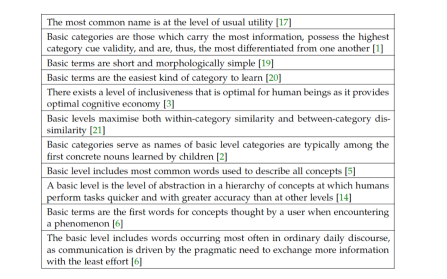
\includegraphics[scale=0.65]{05/basic.png}
    \caption{Alcune definizioni di Basicness.}
    \label{fig:bas}
\end{figure}

\paragraph{Considerazioni:}

\begin{itemize}
  \item Sopravvivenza sociale: l'acquisizione del vocabolario di base è essenziale per i \textit{second language learner} per poter comunicare i propri bisogni. 
  \item Legame termine-concetto: purtroppo non tutti i concetti sono facilmente descritti da un termine. Inoltre alcuni termini basic possono essere usati per concetti avanzati. Per esempio cane che ha un significato in termini militari. 
  \item Soggettività: il livello base è estremamente soggettivo poiché gli stessi termini sono interpretati in maniera diversa da persone diverse. 
  \item Advanced: i termini advanced vengono definiti in materia di basic. Tutto ciò che non è basic è advanced. 
\end{itemize}

\section{Annotazioni e Misure di Agreement}

\qs{}{Cosa significa \fancyglitter{annotare}?}

\begin{itemize}
  \item Etichettare manualmente dei dati (assegnando nomi e categorie). 
  \item Seguire delle linee guida per l'annotazione.
\end{itemize}

\qs{}{Perché si deve annotare?}

\begin{itemize}
  \item Per dare supporto ad affermazioni empiriche. 
  \item Per sviluppare e testare modelli computazionali.
\end{itemize}

\nt{C'è però un problema: non esiste un criterio oggettivo per valutare la validità di un'annotazione.}

\subsection{Introduzione al Problema dell'Annotazione}

\qs{}{Come si valuta l'affidabilità di un'annotazione?}

\begin{itemize}
  \item Più persone effettuano un'annotazione sugli stessi dati seguendo le stesse linee guida. 
  \item Successivamente si calcola l'\fancyglitter{inter-annotator agreement}. 
\end{itemize}

\dfn{Row/Observed Agreement}{
  Un primo criterio per valutare l'agreement è il seguente: numero di items con la stessa etichetta / totale di items annotati (fig: \ref{fig:ag}).
}

\paragraph{Bisogna considerare tre aspetti:}

\begin{itemize}
  \item Problema nei dati: potrebbero essere troppo ambigui. 
  \item Problemi degli annotatori: le linee guida non sono corrette, sono incomplete, etc. 
  \item Il task è troppo difficile: per esempio se si vuole annotare un testo in lingua inglese è necessario farlo fare a madrelingua.
\end{itemize}

\begin{figure}[h]
    \centering
    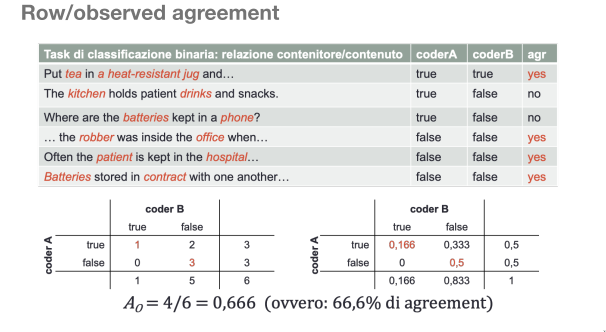
\includegraphics[scale=0.65]{05/ro.png}
    \caption{Esempio di agreement.}
    \label{fig:ag}
\end{figure}

\paragraph{Vantaggi e svantaggi del Row/Observed agreement:}

\begin{itemize}
  \item [\textcolor{green}{\ding{51}}] Facile da misurare e da capire. 
 \item [\textcolor{green}{\ding{51}}] Comunemente usato.
       \item [\textcolor{red}{\ding{55}}] Non tiene conto del caso (chance-aware agreement). 
          \item [\textcolor{red}{\ding{55}}] Un numero di classi (possibili risposte) può risultare in un agreement dovuto al caso più alto. 

             \item [\textcolor{red}{\ding{55}}] Non tiene conto della distribuzione degli item sulle classi. 
\end{itemize}

\subsection{Calcolo dell'Agreement}

\dfn{Agreement con Correzione del Caso}{
  Si calcola la quantità di agreement ottenuto al di sopra del livello di agreement che ci si aspetterebbe da un'annotazione fatta a caso:

  $$R = \frac{A_o - A_e}{1 - A_e}$$

Con:
\begin{itemize}
  \item $A_o$: Observed agreement. 
  \item $A_e$: chance agreement atteso da un'annotazione casuale. 
  \item $1 - A_e$: massimo livello di agreement ottenibile al di sopra del caso. 
  \item $A_o - A_e$: effettivo livello di agreement ottenuto dall'annotazione.
\end{itemize}

}

\paragraph{Le misure di agreement hanno modi diversi di calcolare $A_e$:}

\begin{itemize}
  \item Bennet, Alpert e Goldstein: assumono una distribuzione uniforme. 
  \item Scott: assume una distribuzione unica per tutti gli annotatori. 
  \item Cohen: assume distribuzioni diverse per ogni coder.
\end{itemize}

\dfn{Kappa di Cohen}{
  La K di Cohen assume distribuzioni di probabilità diverse per ogni annotatore. Le distribuzioni possono essere lette ai margini di una tabella di contingenza (fig: \ref{fig:k}). Assumendo che gli annotatori $C_A$ e $C_B$ eseguano l'annotazione in modo indipendente l'uno dall'altro e che $k$ sia una delle possibili categorie, allora:

  $$P(k | C_A) * P(k | C_B)$$

è la probabilità, dovuta al caso, che i due annotatori concordino sulla categoria $k$. Quindi la probabilità di agreement dovuta al caso su tutte le categorie è:

$$\displaystyle\sum_{k \in K} P(k | C_A) * P(K | C_B)$$


}

\begin{figure}[h]
    \centering
    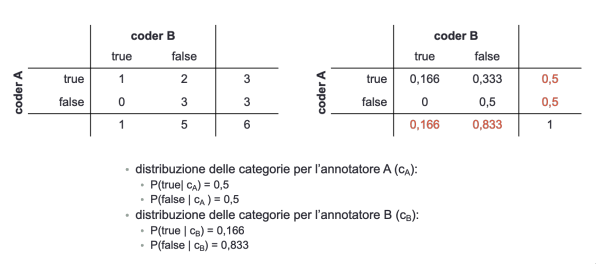
\includegraphics[scale=0.65]{05/k.png}
    \caption{Esempio di K di Cohen.}
    \label{fig:k}
\end{figure}

\nt{Questa misura ha la caratteristica di schiacciare molto l'agreement.}

\begin{figure}[h]
    \centering
    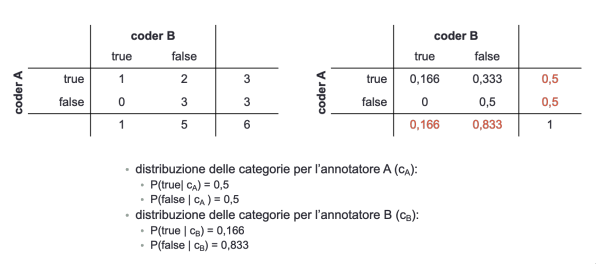
\includegraphics[scale=0.65]{05/k.png}
    \caption{Misura per interpretare i valori di $k$.}
\end{figure}



